
\section{Experiments}
\label{sec:expts}

\begin{figure*}[htb]

  \centering  % centers the image in the column

  % replace the second argument below with your filename. I like to
  % place all my figures in a sub-directory to keep things organized
  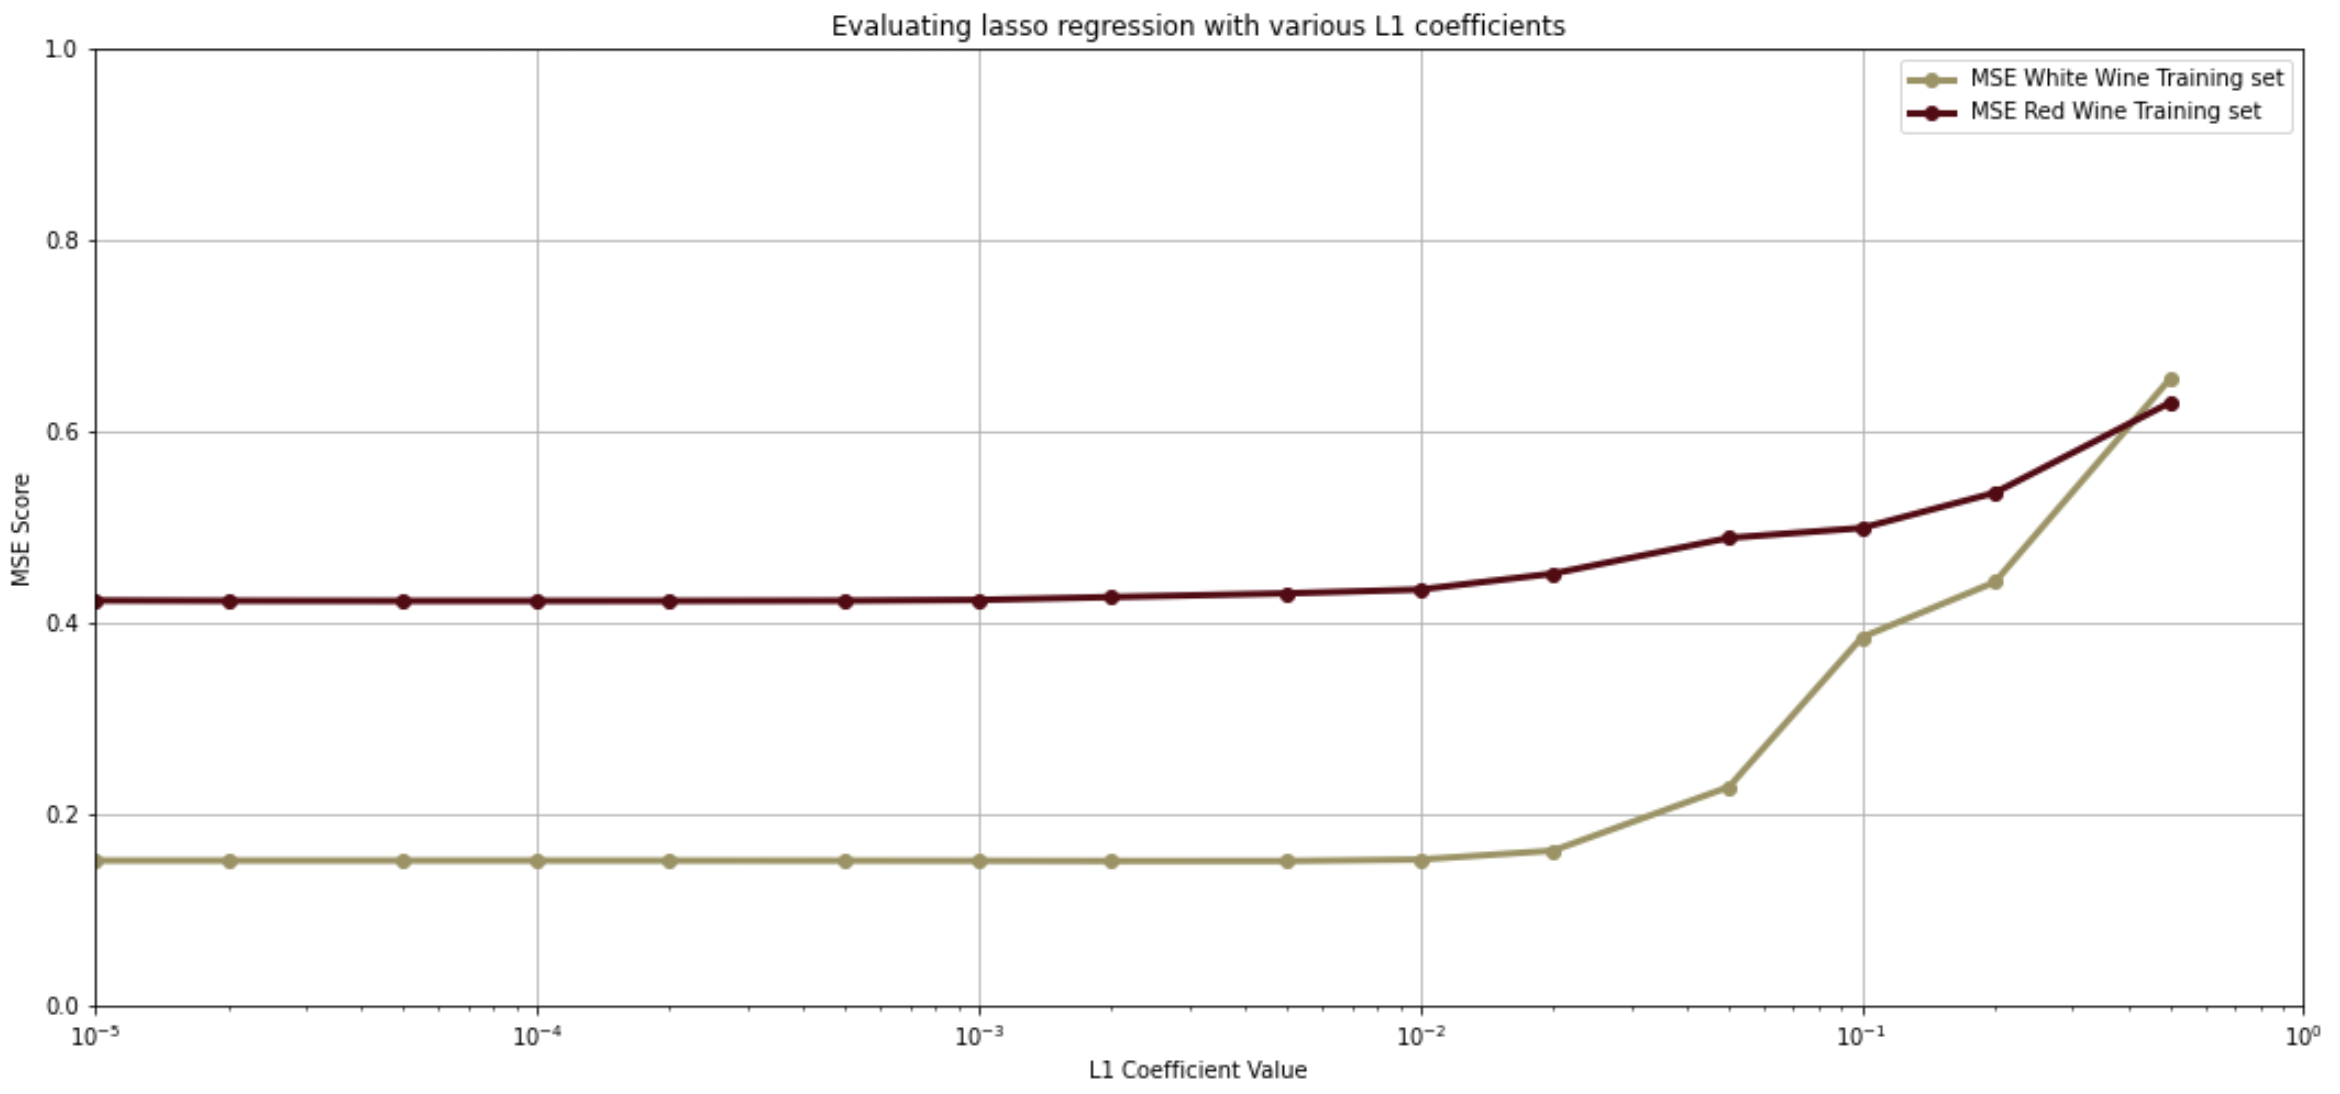
\includegraphics[width=\linewidth]{figs/hptuning.png}

  % *Every* figure should have a descriptive caption.
  \caption{Mean squared error (MSE) by L1 regularization coefficient value for both the red and white wine training sets. The optimal L1 coefficient for the red wine dataset is at 0.00012 with an MSE of 0.424. The optimal L1 coefficient for the white wine dataset is at 0.0024 with an MSE of 0.152. Dark red indicates the red wine dataset, and beige indicates the white wine dataset.}

  % The label is a handle you create so that you can refer to this
  % figure (using the \ref{} command) from other parts of your
  % document. LaTeX automatically renumbers figures and updates
  % references when you recompile, so you should do it this way rather
  % than hard-coding in references. Notice that I've also been
  % creating labels for the various sections in the document; I could
  % use \ref{} command to refer to those sections using their labels
  % too.
  \label{fig:hptuning}

\end{figure*}

We approached this regression problem knowing that we wanted to employ regularization methods in some manner. Regularization simplifies the model by tuning the weights of certain features, and thus reducing the potential for overfitting. Our initial thought was to implement lasso regression, which is particularly successful in multivariate models where some features may play a larger role in predicting the outcome than others. If you visualize each feature holding some weight or coefficient value, lasso regression shrinks these weights all the way to zero on less important features through a process called L1 regularization. Therefore, due to our prior data exploration process, we hypothesized that some variables would have stronger correlations with wine rating than others, so feature selection was an important consideration for our choice of model. \\\\
We compared this to another common regression technique known as ridge regression which implements a slightly different regularization method that shrinks weights but doesn’t set them to zero. The weights of features in ridge regression never reached zero, while they often did in our lasso models, which match the proper functionalities of the two types of regression. Despite converging on different L1 regularization coefficients, the mean squared error of each type of regression was comparable and did not indicate a strong difference in their coefficients of determination. However, we decided to move forward with the lasso approach due to what we know about its built-in feature selector properties. \\\\
After settling on lasso regression, we turned to the Lasso structure as a part of \textit{scikit-learn}’s linear modeling package. Lasso regression adopts coordinate descent as its optimizer and tunes learning rate automatically. We performed 5-fold cross validation on our training data, using mean squared error as our scoring metric. In terms of hyperparameters in question, our main focus was on optimizing the L1 regularization coefficient. This would determine the degree at which certain features were rejected from the model. We tuned this value through built-in grid search functionality to optimize the mean squared error of the model (seen in figure~\ref{fig:hptuning}). \\\\
For the red wine dataset, the mean squared error over the 5-fold cross validation data was 0.424 and the optimal L1 coefficient was 0.00012. For the white wine dataset, the mean squared error was 0.152 and the optimal L1 coefficient was 0.0024. After finding the ideal L1 coefficient, we fit our models to the training and test datasets and evaluated them by the coefficient of determination. \\\\